\chapter{Principy a historie regulárních výrazů}\label{sec:Principle}

Tato kapitola se zabývá definicí regulárních výrazů, jejich fungováním a jak se jednotlivé implementace mohu lišit. 
Součástí jejich implementace provází několik pojmů z~teoretické informatiky, odkud pocházejí.
Hlavně se jedná o~\textbf{Konečné automaty} a \textbf{Thompsonovo sestrojení}.

\section{Formální jazyk}
Formální jazyk je libovolná množina konečných slov nad určitou abecedou \cite{MUNIFL}. 
Slova chápeme jako řetězce znaků, která jsou přijímaná zadaným jazykem.
Délka slov musí být sice konečná, ale množina těchto slov může být nekonečná. 
Tyto jazyky mohou být například definovány regulárními výrazy, formální gramatikou nebo konečnými automaty. 

\section{Konečný automat}\label{sec:FiniteAutomaton}
S~regulárními výrazy se často pojí konečné automaty, jedná se o~další oblast z~teoretické informatiky.
Tato práce implementuje regulární výrazy právě ve formě konečných automatů.
Zjednodušeně se dá říct, že konečný automat je výpočetní model jednoduchého počítače, který má určitý počet stavů a přechodů \cite{Havrlant}. 

Konečné automaty se dělí na \textbf{deterministické} a \textbf{nedeterministické}, zkráceně \textbf{DKA} (deterministický konečný automat) a \textbf{NKA} (nedeterministický konečný automat).
DKA mohou mít v~daném stavu pro každý znak abecedy \textbf{právě jeden} přechod, zatímco NKA umožňují více stejných přechodů z~daného stavu. 
NKA také mohou obsahovat tzv.\ prázdný znak často označovaný řeckým písmenem epsilon $\varepsilon$. 
Prázdné znaky slouží pro změnu stavu bez změny aktuální pozice ve hledaném slově. 
Také platí, že každý NKA je možné převést na ekvivalentní DKA.
Formální definice těchto automatů následuje níže.

\newpage

\noindent Deterministický konečný automat je pětice $(Q, \Sigma, \delta, q_0, F)$\cite{Viswanathan_2017}:
\begin{itemize}
	\item $Q$ --- konečná množina stavů.
	\item $\Sigma$ --- konečná vstupní abeceda.
	\item $\delta: Q \times \Sigma \rightarrow Q$ --- přechodová funkce.
	\item $q_0 \in Q$ --- počáteční stav.
	\item $F \subseteq Q$ --- množina konečných stavů.
\end{itemize}

\noindent Nedeterministický konečný automat je pětice $(Q, \Sigma, \Delta, S, F)$\cite{Viswanathan_2017}:
\begin{itemize}
	\item $Q$ --- konečná množina stavů.
	\item $\Sigma$ --- konečná vstupní abeceda.
	\item $\Delta: Q \times \Sigma \rightarrow 2^Q$ --- přechodová funkce, kde stav a vstupní symbol určuje množinu možných následujících stavů.
	\item $S \subseteq Q$ --- množina počátečních stavů.
	\item $F \subseteq Q$ --- množina konečných stavů.
\end{itemize}

\subsection*{Vizualizace}

Stavy jsou typicky zakreslovány jako kružnice. 
Konečné stavy se označují jako kružnice s~dvojitou čárou. 
Počáteční stavy jsou označovány jako stav, do kterého vede šipka, která ale nevychází z~jiného stavu.
Přechody jsou znázorněny jako šipky vedoucí z~jednoho stavu do druhého a jsou označeny přechodovým symbolem.
Pro upřesnění, přechod může odkazovat na stejný stav ze kterého vychází.
Tyto přechody nám říkají, že pokud chceme přejít z~jednoho stavu do druhého, tak se musíme v~přijímaném slově posunout o~přechodový symbol. 
Pokud to není možné, tak nelze tímto přechodem přejít do tohoto stavu.
Pro ukázku lze porovnat dva ekvivalentní konečné automaty, NKA na obrázku~\ref{fig:NFAex} a DKA na obrázku~\ref{fig:DFAex}.

\begin{figure}[!h]
	\centering
	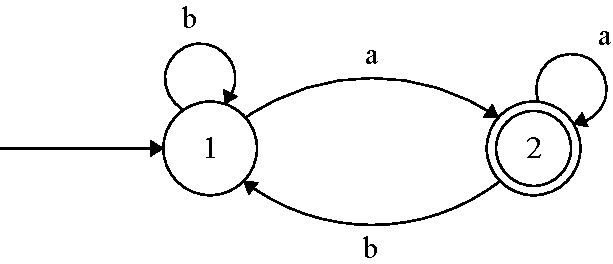
\includegraphics[width=0.45\textwidth]{Figures/DFA_example.pdf}
	\caption{Příklad deterministického automatu přijímající slova obsahující písmena z~abecedy \{a, b\} končící písmenem a}
	\label{fig:DFAex}
\end{figure}

\begin{figure}[!h]
	\centering
	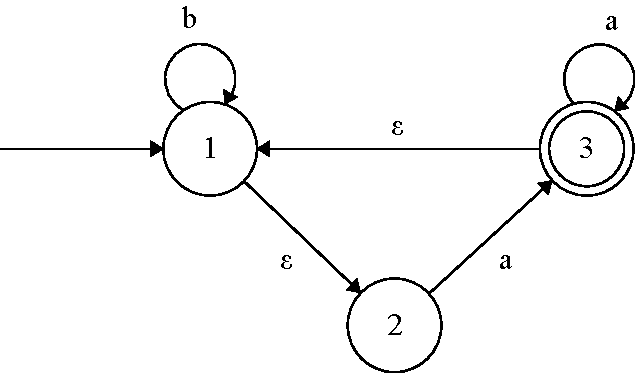
\includegraphics[width=0.45\textwidth]{Figures/NFA_example.pdf}
	\caption{Příklad nedeterministického automatu ekvivalentního k~předchozímu deterministickému}
	\label{fig:NFAex}
\end{figure}

\section{Bezkontextová gramatika}
Součástí této práce je i využití Bezkontextové gramatiky, pro nadefinování syntaxe regulárních výrazů.

Bezkontextová gramatika je jedna z~dalších formálních gramatik, kterými lze definovat formální jazyky. 
Je určená konečnou množinou \textbf{neterminálních symbolů} (proměnných), konečnou množinou \textbf{terminálních symbolů}, která nesmí mít žádné prvky společné s~předchozí množinou.
Dále je součástí \textbf{počáteční neterminál}, s~konečnou množinou \textbf{přepisových pravidel}\cite{MUNIFL}.

Pro příklad může sloužit výraz $A \longrightarrow \beta$, kde A~je neterminál a $\beta$ je řetězec složený z~terminálů a/nebo neterminálů. 
Dále šipka indikuje \textbf{přepsání} tzn. levá strana se přepisuje na stranu pravou.
Konečný řetězec generovaný danou gramatikou, je pouze tvořen terminálními symboly.
Aby mohl být řetězec přijímaný zadanou gramatikou, musí ho být schopná vygenerovat.

Na obrázku \ref{fig:CFG} se nachází příklad bezkontextové gramatiky.
Ta přijímá slova, které obsahují buď sekvenci písmen \textit{a} následující sekvenci písmen \textit{b}, anebo naopak.
Vstupním neterminálem této gramatiky je symbol \texttt{S}.
Příkladem vstupu může být řetězec \textit{aabb}, jehož zpracování je následující:

\texttt{$S \rightarrow AB \rightarrow AaB \rightarrow aaB \rightarrow aaBb \rightarrow aabb$}

Ve zpracování šipka signalizuje přepis jednoho z~neterminálu na jeden z~jeho možných výběrů.
Pokud je výsledek shodný s~hledaným řetězcem, tak vyhledání proběhlo úspěšně.

\begin{figure}[!h]
	\centering
	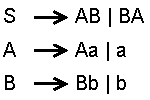
\includegraphics[width=0.17\textwidth]{Figures/CFG.pdf}
	\caption{Příklad jednoduché bezkontextové gramatiky}
	\label{fig:CFG}
\end{figure}


\section{Vznik, implementace a vzory}
Regulární výrazy byly poprvé nadefinovány Americkým matematikem \textbf{Stephan Cole Kleenem}, jako regulární události (regular events)\cite{Leung_2010, Kleene_1951}. 
Dále se staly součástí teoretické informatiky, jako podkategorie \textbf{teorie automatů}.
Ačkoliv byly nadefinovány začátkem padesátých let, tak jejich využití v~počítačích nastalo až na konci šedesátých let a to v~jednom z~nejznámějších operačních systémů UNIX.

\subsection*{Thompsonovo sestrojení}

První, kdo navrhl implementaci používanou v~počítačích, byl \textbf{Ken Thompson}\cite{ScanToPDF}.
Principem byl převod regulárního výrazu na NKA.
Tato metoda se často používá doposud, v~podobné či nezměněné podobě.
Algoritmus se pojmenoval \textbf{Thompson's construction} (Thompsonovo sestrojení), který převádí textovou reprezentaci výrazu na ekvivalentní nedeterministický automat.
Toto sestrojení je využito v~této práci a blíže jej popisuje následující část textu.

Převod na NKA se běžně využívá, jelikož je poměrně jednoduchý na implementaci.
Thompsonovo sestrojení poskytuje řešení, jak tento převod uskutečnit.
Konečné automaty jsou vhodnou formou reprezentace regulárních výrazů, protože mohou být na počítačích rychle vyhodnoceny.
NKA je sice obecně pomalejší oproti jeho ekvivalentního DKA, ale jelikož dnešní formy výrazů umožňují složitější konstrukce, tak nelze vždy použít převod na DKA.
Hlavním důvodem je, že NKA na rozdíl od DKA umožňuje backtracking (zpětné sledování), kterého může být využito pro složitější operace, jako je look-around (rozhlédnutí se kolem sebe).
Backtracking znamená, že pokud se NKA nachází ve stavu, ze kterého nelze pokračovat dále, tak je potřeba se vrátit do předchozího stavu.
V~NKA se tohoto využívá, jelikož neexistuje jednoznačná cesta vyhodnocení.
DKA mají výhodu, že jsou rychlejší, ale také jsou typicky mnohem větší než jejich ekvivalentní NKA.
Dnes se ale často využívá kombinace DKA a NKA, kdy DKA se využije, pokud je to možné, jinak se využije NKA.

Výsledný NKA po Thompsonově sestrojení má právě jeden vstupní a výstupní stav. 
Thompsonovo sestrojení dále definuje několik následujících pravidel.

Prázdný výraz \textit{$\varepsilon$}, je převedený na vstupní stav, přechod \textit{$\varepsilon$} a konečný stav.
Výsledný konečný automat je na obrázku~\ref{fig:NFAepsilon}.
\begin{figure}[!h]
	\centering
	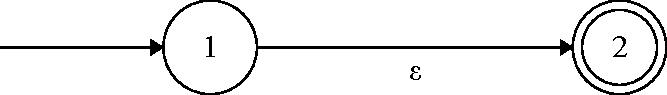
\includegraphics[width=0.45\textwidth]{Figures/NFA_epsilon.pdf}
	\caption{Převedený prázdný výraz $\varepsilon$}
	\label{fig:NFAepsilon}
\end{figure}

Výraz \texttt{a}, je převedený podobně jako prázdný výraz, ale s~rozdílem přechodu \textit{a} místo \textit{$\varepsilon$}.
Konečný automat, který tímto převodem vznikne je ukázán na obrázku~\ref{fig:NFAa}.
\begin{figure}[!h]
	\centering
	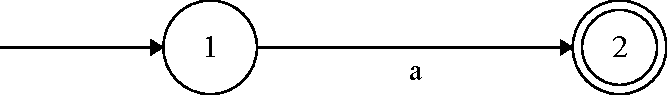
\includegraphics[width=0.45\textwidth]{Figures/NFA_a.pdf}
	\caption{Převedený výraz \texttt{a}}
	\label{fig:NFAa}
\end{figure}

Pro zadaný výraz \texttt{s|t} (varianta), kde \textit{s} je levá strana varianty a \textit{t} je pravá strana varianty, platí, že ze stavu \textit{q} (počáteční stav) vedou dva přechody
\textit{$\varepsilon$}, na počáteční stavy variant \textit{s} a \textit{t}. 
Z~těchto počátečních stavů dále pokračuje sekvence stavů \textit{N(s)} pro \textit{s} a \textit{N(t)} pro \textit{t}.
Konce variant \textit{s} a \textit{t} mají každé jediný přechod \textit{$\varepsilon$} na konečný stav \textit{f}.
Na obrázku~\ref{fig:NFAunion} je znázorněný výsledný NKA, kde skupina stavů v~zelené části je \textit{s} a červená skupina je \textit{t}.
\begin{figure}[!h]
	\centering
	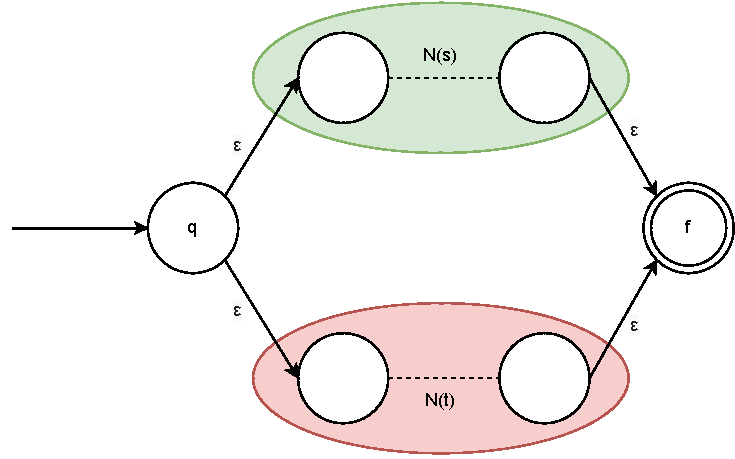
\includegraphics[width=0.6\textwidth]{Figures/NFA_union.pdf}
	\caption{Převedený výraz \texttt{s|t}}
	\label{fig:NFAunion}
\end{figure}

Další pravidla pro sestrojení lze například najít v~následujících článcích \cite{Thompson1,Thompson2}.
Některé pravidla jsou v~této práci upravená, ale fungují na stejném principu.

\subsection*{Základní vzory regulárních výrazů}
V~předchozích sekcích již byly popsány základní konstrukce týkající se regulárních výrazů.
Tato sekce se zabývá jejich základními vzory, neboli jejich formou zápisu a syntaxí.
Popis následujících vzorů vychází ze syntaxe regulárních výrazů pro jazyk JavaScript.

Za nejjednodušší výraz lze považovat prázdný výraz, také označovaný jako $\varepsilon$. 
Tento výraz dokáže přijímat slova délky 0, resp. prázdná slova.
Výrazy mohou obsahovat \textbf{téměř} libovolný znak, který bude přijímat slova s~tímto znakem. 
Avšak nemohou být použity znaky, které jsou rezervované, neboli jsou součástí syntaxe regulárních výrazů.
Chceme-li použít tyto znaky, je potřeba použít zpětné lomítko \texttt{\textbackslash}. 
Takové spojení znaku a zpětného lomítka se pak anglicky nazývá \textbf{escaped character}.
Také existují znaky, které nejsou součástí rezervovaných znaků, ale lze před nimi použít zpětné lomítko.
Funkcionalita těchto znaků se následně mění, např. pokud použijeme zpětné lomítko před znakem \textit{d}, tak to ve výrazu značí přijmutí čísla od 0 do 9.

Iterace je možnost jak lze opakovaně provádět nějaký vzor.
Například lze iterovat znak, skupinu a další konstrukce. 
Nelze však opakovat jakýkoliv vzor.
Prvním typem iterace je \texttt{\textbf{*}}, známa jako \textbf{Kleene star}.
Tento druh iterace může mít počet opakování od \textbf{0} do \textbf{n}. 
Dále existují další 2 typy iterací, a to je iterace v~rozmezí $1-n$ označována znakem \texttt{+} a \textit{iterace v~rozmezí}, která se značí \{od,do\}.
V~regulárních výrazech se vždy vzor opakování vyskytuje za konstrukcí, které se má opakovaně provádět.

Operace \textit{varianta} je dalším základním vzorem pro regulární výrazy. 
Jedná se o~výběr mezi pravou a levou stranou. 
Oddělovacím znakem je typicky \texttt{|} podobně jako bitová operace \textit{OR} v~mnoha programovacích jazycích.

Dalšími základními konstrukty jsou například skupiny, které jsou obaleny v~jednoduchých závorkách.
Ty slouží k~rozdělení částí regulárních výrazů, které jsou po dokončení vyhledávání přístupné jako oddělené části vyhledání.

Příkladem regulárního výrazu z~JavaScriptové syntaxe může být výraz \texttt{\textasciicircum \textbackslash d\{3\}(~?\textbackslash d\{3\})\{2\}\$}, který přijímá telefonní čísla.
Znak \texttt{\textasciicircum} znamená, že se musí jednat o~začátek textového řetězce a znak \texttt{\$} naopak znamená konec řetězce.
Dále symbol \texttt{?} znázorňuje nepovinnost vzoru, který se před ním nachází.
První část \texttt{\textasciicircum \textbackslash d\{3\}} přijímá první tři číslice telefonního čísla.
Dále \texttt{(~?\textbackslash d\{3\})\{2\}\$} přijímá dalších šest číslic z~telefonního čísla, kde jednotlivé trojčíslí mohou být odděleny mezerou.
Příkladem přijímaného řetězce může být \textit{123 456 789}.
Jak je patrné, tak tento konkrétní výraz nepokrývá telefonní čísla s~předčíslím.

Na obrázku \ref{fig:REGEXEXMP} lze vidět příklad regulárního výrazu, ve kterém jsou použity a popsány některé ze zmíněných vzorů.

\begin{figure}[!h]
	\centering
	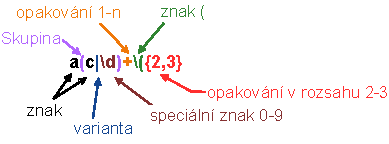
\includegraphics[width=0.5\textwidth]{Figures/regex_exmp.pdf}
	\caption{Příklad regulárního výrazu}
	\label{fig:REGEXEXMP}
\end{figure}

\subsection*{Implementace v~programovacích jazycích}\label{sec:impipl}

V~dnešní době mají v~podstatě skoro všechny programovací jazyky nějakou formou implementované regulární výrazy.
Implementace v~programovacích jazycích se často liší svou syntaxí a obsáhlostí, ale jejich základ bývá stejný.
Může se tak stát to, že funkcionalita podporována jedním jazykem není podporovana druhým.
Taktéž oproti původním regulárním výrazům, dnešní implementace obsahují mnohdy složitější koncepce, jako je look-around nebo například rekurze.
Někdy jazyky sice sdílí stejné konstrukce, ale mohou se lišit syntaxí.

Look-around je již celkem pokročilá funkcionalita, jejímž principem je takzvané nezachytávání znaků při zpracovávání.
Typicky je dělíme podle směru, a to na \textit{dopředné} a \textit{zpětné}.
Pak je dělíme podle podmínění, a to na \textit{kladné} a \textit{negativní}.
Pokud máme kladné podmínění, \textbf{musí} být uzavřený výraz splněný a pokud máme záporné, tak \textbf{nesmí} být splněný.
V~původní formě regulárních výrazů tato funkce neexistovala.

Mnohdy je potřeba nalezený řetězec rozdělit do skupin.
Skupiny mohou být použity pro získání strukturovaných dat nebo pro obalení logického celku, na který lze aplikovat některé operátory, jako je třeba iterace.
Příkladem strukturovaných dat může být vyhledání jména, které lze rozdělit na křestní jméno a příjmení.
Za pomocí skupin lze získat tyto jednotlivé části po dokončeném vyhledání. 
Chceme-li zdůraznit, že zadaný podvýraz je skupinou, obalíme ho do závorek.
Tato vlastnost je důležitá, jelikož není potřeba v~již nalezeném řetězci hledat další podřetězce pomocí dalšího výrazu.
Skupiny se dělí na zachytávající (capturing), pojmenované (named) a nezachytávající (non-capturing).
Pojmenované patří pod zachytávající, akorát jsou identifikovány pomocí názvu místo indexu.
Obě skupiny zůstávají zachycené po dokončeném vyhledávání.
Nezachytávající skupiny slouží čistě pro regulární výrazy, například při opakování části výrazu, ale ve výsledku vyhledání se již nenachází.

Asi nejobsáhlejší implementací je \textit{PCRE} (Perl-Compatible Regular Expressions) a \textit{PCRE2}.
Tento standard pochází z~jazyka Perl, ale také je například součástí jazyka PHP.
Nachází se zde již poměrně složité vzory, jako jsou podmínky nebo rekurze.

\endinput
